\section{PDDL definition}

\subsection{Catching mice}

\begin{figure}[ht]
    \centering
    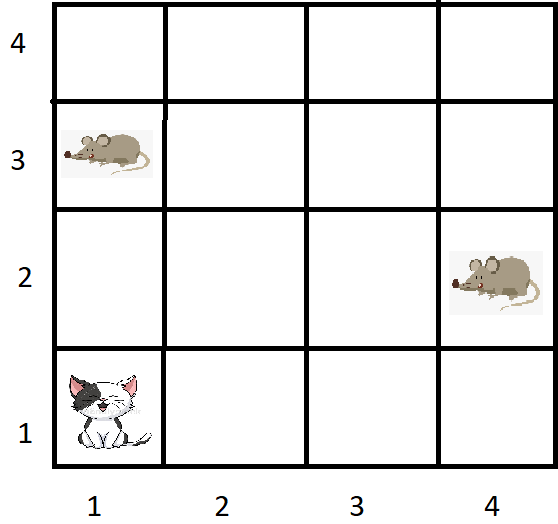
\includegraphics[width=.5\linewidth]{fig/A3/cat_01.png}
    \caption{Problem 1: Catching two mice}
    \label{fig:cat_01}
\end{figure}

The first step to solve the problem is to define the two fundamental actions the cat can take: moving to neighboring rooms and eating a mouse.


\subsubsection{Domain}

The first types of the domain represent the type of elements that can be inside a room: cat and mouse. The square type represents a room, identified by the row and column indices.

The \verb|at| predicate shows whether an object is inside a given room or not. The \verb|adj| predicate indicates whether two squares are adjacent or not. Finally the \verb|dead| predicate shows whether the given mouse is dead or not.


\lstinputlisting[caption=Domain: types and predicates,firstline=1,lastline=8]{../planning/cat-eat.pddl}

To move from one square to another, the two squares must be adjacents to each other, and the cat should be inside the first one. Moving means to leave the current square and to enter the next one.

\lstinputlisting[caption=Domain: the move action,firstline=10,lastline=20]{../planning/cat-eat.pddl}

The cat can eat a mouse when they are both in the same square. Eating a mouse means to remove it from the world and mark it dead.

\lstinputlisting[caption=Domain: the eat action,firstline=22,lastline=32]{../planning/cat-eat.pddl}


\subsubsection{Problem}

The first problem is to catch two mice. There are no constraints besides the rule of moving only to adjacent cells. The initial state can be seen on figure \ref{fig:cat_01}.

The objects that appear in the problem are: a cat, two mice and 16 squares.

\lstinputlisting[caption=Problem: objects,firstline=1,lastline=11]{../planning/cat-p01.pddl}

To describe the initial state, first we must define the adjacency relationship between the squares.

\lstinputlisting[caption=Problem: adjacency relationships,firstline=13,lastline=38]{../planning/cat-p01.pddl}

Then the initial locations of the cat and the mice are specified:

\lstinputlisting[caption=Problem: initial locations,firstline=40,lastline=45]{../planning/cat-p01.pddl}

Finally the goal is defined: to get rid of all the mice.

\lstinputlisting[caption=Problem: goal,firstline=48,lastline=48]{../planning/cat-p01.pddl}


\subsubsection{Result}

One should type the following line to run the example: 

\begin{lstlisting}
fd cat-eat.pddl cat-p01.pddl --heuristic "h=ff( )" --search "astar(h)"
\end{lstlisting}

The program prints the following solution:

\lstinputlisting[caption=Output plan]{../planning/cat-p01-plan.txt}

\begin{figure}[ht]
    \centering
    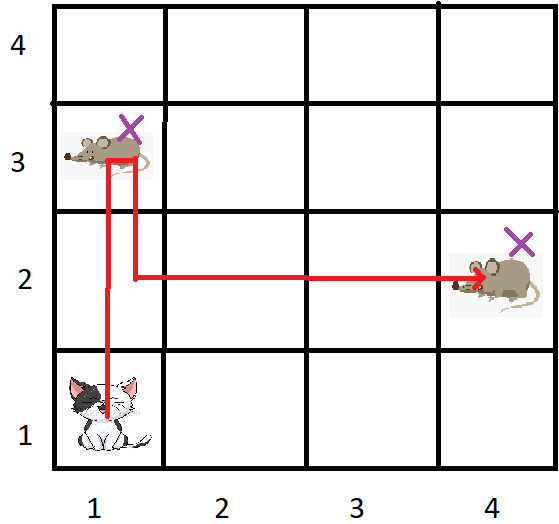
\includegraphics[width=.5\linewidth]{fig/A3/cat_01_sol.png}
    \caption{Problem 1: The resulted plan. The red line shows the trajectory of the cat. The purple 'x' marks that the cat ate the mouse}
    \label{fig:cat_01_sol}
\end{figure}

Figure \ref{fig:cat_01_sol} visualizes the resulted plan. The cat goes straight to the closest mouse, eats it, than moves on the shortest path to the second one and eats it too.






\subsection{Adding walls}












\subsection{Disabling traps}

For making the problems harder, we created a bigger field, containing 36 fields. We also introduced the ability to disable traps.

From now on, we introduce a new domain, which contains some additional actions: grabbing a mouse and disabling the trap with it.
In order to pass through a trap, the cat has to grab a mouse instead of eating it, and throw it in the trap this way, the trap will not act on the cat, so it is as if it does not exist. 

The grab and disable actions were defined as follows:

\begin{lstlisting}
(:action grab
        :parameters (?c - cat ?s - square ?m - mouse)
        :precondition (and 
            (not (dead ?c))
            (at ?m ?s) 
            (at ?c ?s)
            (not (exists (?m1 - mouse) (has ?c ?m1)))
        )
        :effect (and 
            (not (at ?m ?s)) 
            (has ?c ?m)
        )
    )
\end{lstlisting}

\begin{lstlisting}
(:action disable-trap
        :parameters (?c - cat ?s1 - square ?s2 - square ?m - mouse ?t - trap)
        :precondition (and 
            (not (dead ?c))
            (adj ?s1 ?s2)
            (at ?c ?s1)
            (at ?t ?s2)
            (has ?c ?m) 
        )
        :effect (and 
            (not (at ?t ?s2)) 
            (dead ?m)
            (not (has ?c ?m))
        )
    )
\end{lstlisting}


\subsubsection{First example}
In this example we have 8 mice, 5 traps and 5 walls. Here the cat is forced only once to disable a trap. When passing past the mouse at (5,1) the cat is forced to grab the mouse, to disable the trap at (6,1) to reach the mouse at (6,2).

\begin{figure}[ht]
    \centering
    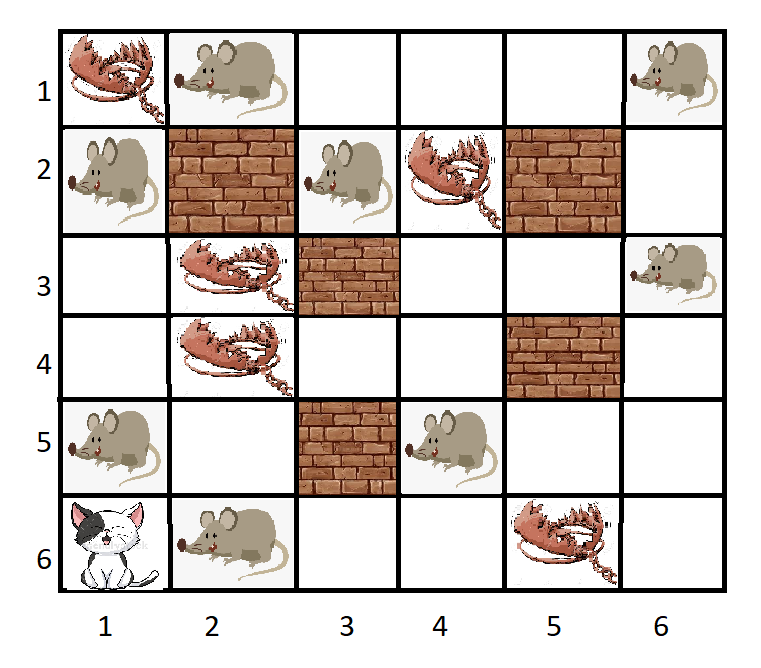
\includegraphics[width=.5\linewidth]{fig/A3/cat_08.png}
    \caption{Problem 9: Catching eight mice, disabling traps, avoid walls }
    \label{fig:cat_08}
\end{figure}


\begin{figure}[ht]
    \centering
    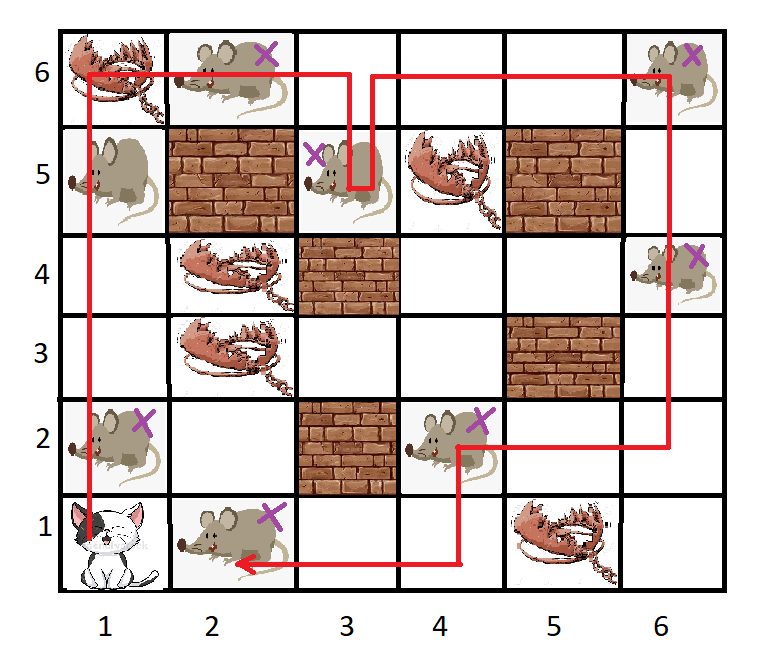
\includegraphics[width=.5\linewidth]{fig/A3/cat_08_sol.png}
    \caption{Problem 9: Catching five mice, disabling traps, avoid walls }
    \label{fig:cat_08_sol}
\end{figure}

\subsubsection{Second example}

\begin{figure}[ht]
    \centering
    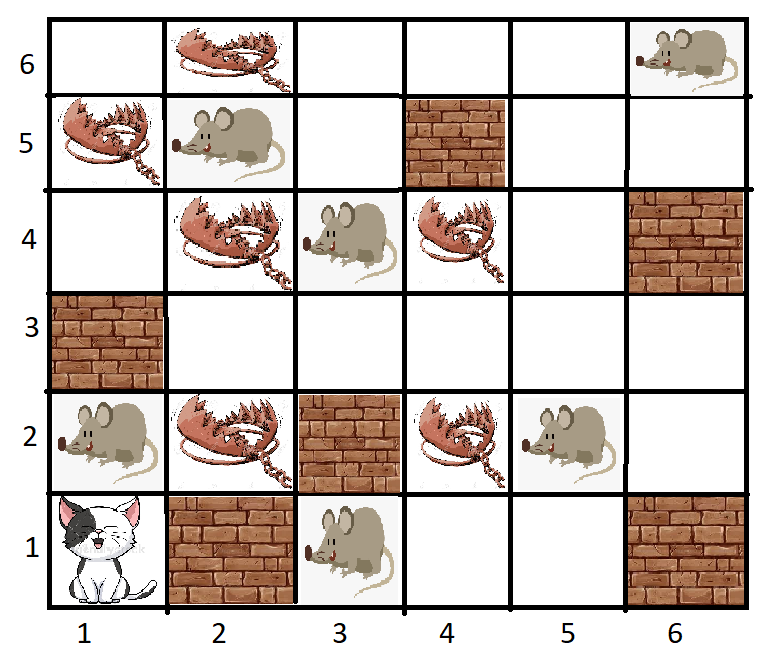
\includegraphics[width=.5\linewidth]{fig/A3/cat_09.png}
    \caption{Problem 9: Catching five mice, disabling traps, avoid walls }
    \label{fig:cat_09}
\end{figure}



The solution can be found below, where the mouses marked with a purple X were eaten by the cat, the other one were 'thrown' into the trap, so the cat could pass through it:



\begin{figure}[ht]
    \centering
    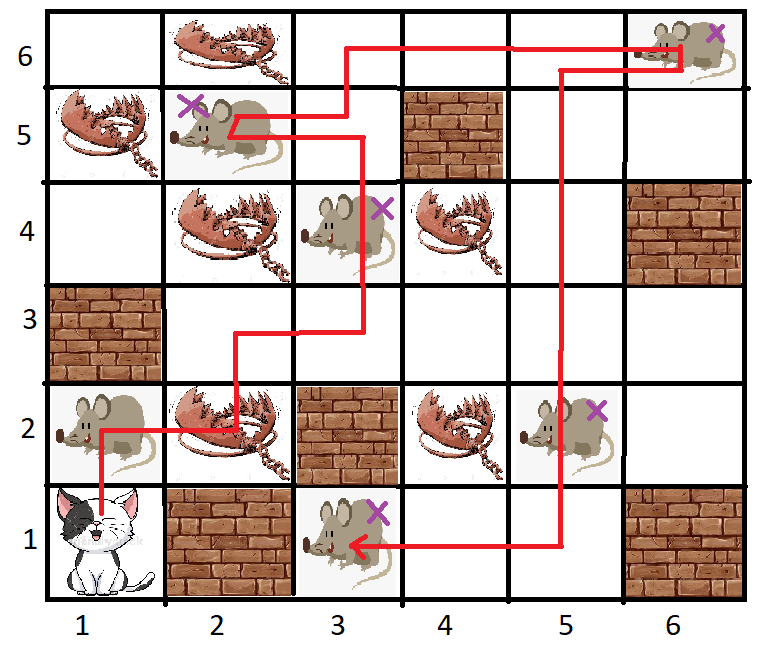
\includegraphics[width=.5\linewidth]{fig/A3/cat_09_sol.png}
    \caption{Problem 9 solution}
    \label{fig:cat_09_sol}
\end{figure}


As we can see, in the first step, the cat having no other option, it had to grab the mouse at (2,1) and throw it into the trap at (2,2) so that it could go forward to eat the other mice.



\subsubsection{Third example}

\begin{figure}[ht]
    \centering
    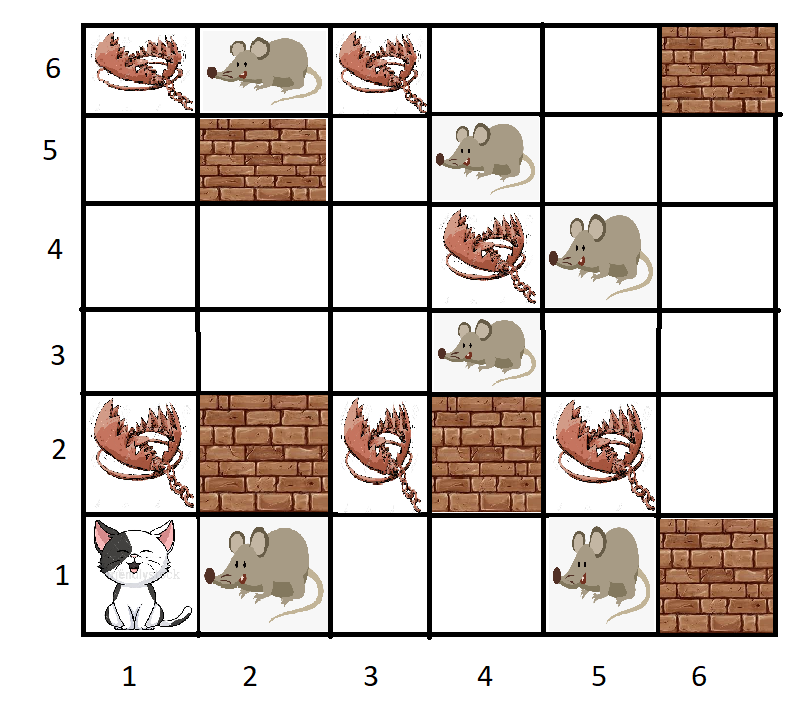
\includegraphics[width=.5\linewidth]{fig/A3/cat_10.png}
    \caption{Problem 10: Catching five mice, disabling traps, avoid walls }
    \label{fig:cat_10}
\end{figure}

In this example, the cat is trapped in the first row, so it is forced to throw a mouse in one of the traps from the second row. Similarly in the sixth row, the mouse is place between two traps and a wall, so the cat is forced to disable one of the traps, using a mouse.
Below we can see the found solution:


\begin{figure}[ht]
    \centering
    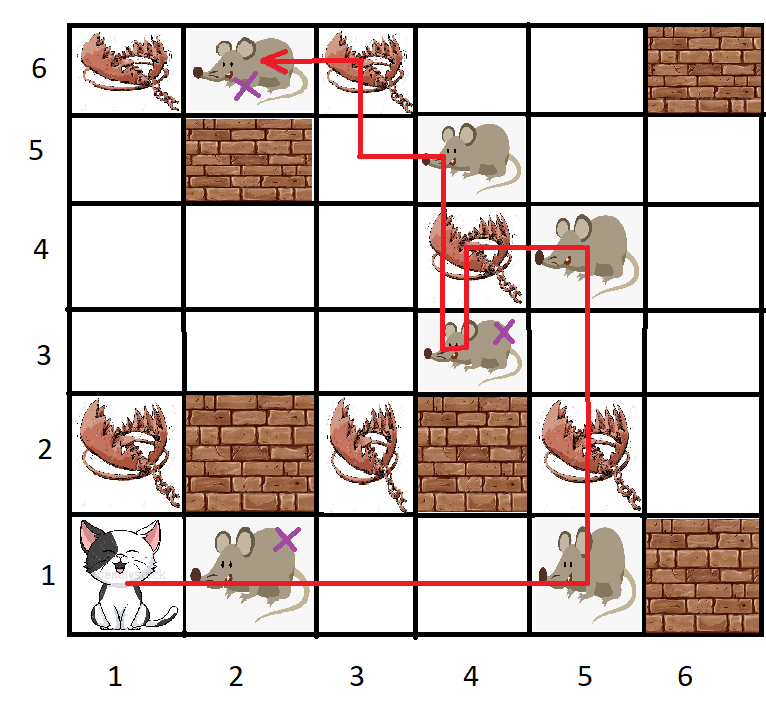
\includegraphics[width=.5\linewidth]{fig/A3/cat_10_sol_withoutWeight.png}
    \caption{Problem 10 solution}
    \label{fig:cat_10_solution}
\end{figure}


\subsubsection{Third example with actions having costs}
We also implemented the second examples with actions that have costs, to force the fast downward planner to search for the optimal solution.
The costs of the actions were implemented as follows:



\begin{lstlisting}
(:functions
        (total-cost)
    )

    (:action move
        :parameters (?c - cat ?s1 - square ?s2 - square)
        :precondition (and 
            (not (dead ?c))
            (adj ?s1 ?s2)
            (at ?c ?s1)
            (not (exists (?w - wall) (at ?w ?s2)))
        )
        :effect (and 
            (not (at ?c ?s1))
            (when (exists (?t - trap) (at ?t ?s2)) (dead ?c))
            (when (not(exists (?t - trap) (at ?t ?s2))) (at ?c ?s2))
            (increase (total-cost) 50)
        )
    )
  
    (:action eat
        :parameters (?c - cat ?s - square ?m - mouse)
        :precondition (and 
            (not (dead ?c))
            (at ?m ?s) 
            (at ?c ?s)
            (not (exists (?m1 - mouse) (has ?c ?m1)))
        )
        :effect (and 
            (not (at ?m ?s)) 
            (dead ?m)
            (increase (total-cost) 0)
        )
    )

    (:action grab
        :parameters (?c - cat ?s - square ?m - mouse)
        :precondition (and 
            (not (dead ?c))
            (at ?m ?s) 
            (at ?c ?s)
            (not (exists (?m1 - mouse) (has ?c ?m1)))
        )
        :effect (and 
            (not (at ?m ?s)) 
            (has ?c ?m)
            (increase (total-cost) 50)
        )
    )

    (:action disable-trap
        :parameters (?c - cat ?s1 - square ?s2 - square ?m - mouse ?t - trap)
        :precondition (and 
            (not (dead ?c))
            (adj ?s1 ?s2)
            (at ?c ?s1)
            (at ?t ?s2)
            (has ?c ?m) 
        )
        :effect (and 
            (not (at ?t ?s2)) 
            (dead ?m)
            (not (has ?c ?m))
            (increase (total-cost) 50)
        )
    )
\end{lstlisting}


Each action has a cost of 50, except for the eat action, which has 0 cost. Below we can see the solution for the weighted actions:

\begin{figure}[ht]
    \centering
    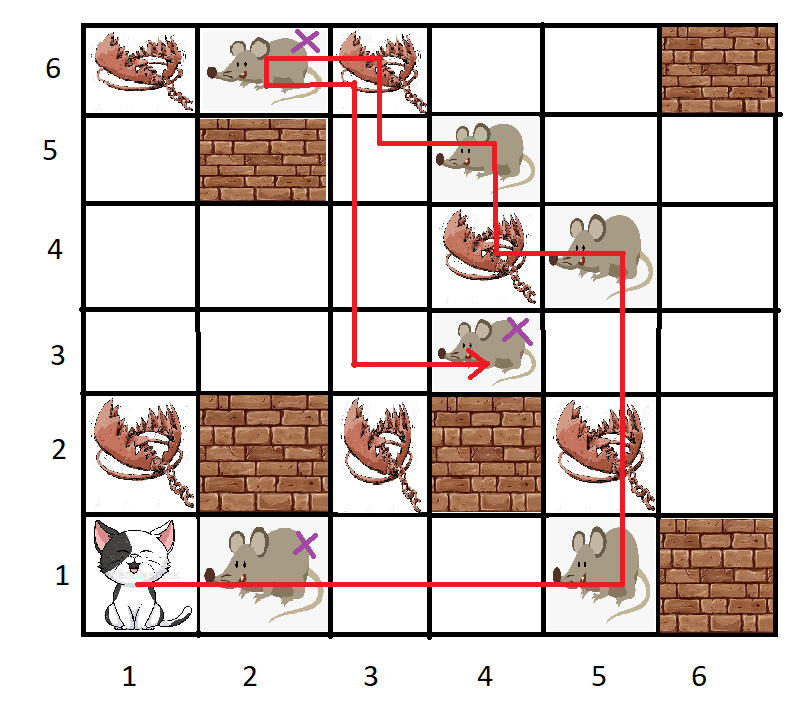
\includegraphics[width=.5\linewidth]{fig/A3/cat_10_withWeigth.png}
    \caption{Problem 10 solution with weighted actions}
    \label{fig:cat_10_solution_withWeights}
\end{figure}


As it can be seen, after disabling the trap at (4,4) the cat did not eat the mouse at (3,4) but grabbed the mouse at (5,4) instead and went to disable the trap at (6,3), ate the mouse at (6,2) and only after that it went back to eat the mouse at (3,4)
